\section{Desarrollo}

\begin{definition}[División con resto]
    Para cualesquiera dos polinomios $F(x)$ y $G(x)$ existen dos los polinomios únicos $Q(x)$ y $R(x)$, tal que
    \[
        F(x) = G(x)Q(x) + R(x),\ \text{con}\ 0 \leq \deg{R(x)} < \deg{G(x)}.
    \]
    Donde el \emphtext{cociente} y el \emphtext{resto} (o \emphtext{residuo}) de la división son $Q(x)$ y $R(x)$, respectivamente.
    Cuando $R(x) = 0$, diremos que $G(x)$ divide a $F(x)$, y lo vamos a denotar como $G(x) \mid F(x)$.
\end{definition}
Por ejemplo, con $F(x) = x^7 - 1$ y $G(x) = x^3 + x + 1$ llegaremos a que
\[
    x^7 - 1 = (x^3 + x + 1)(x^4 - x^2 - x + 1) + (2 x^2 - 2).
\]
Con cociente $Q(x) = x^4 - x^2 - x + 1$ y resto $R(x) = 2 x^2 - 2$.
Para abreviar, diremos $G(x) \mid F(x)$ como $G \mid F$, puesto que en una división de polinomios los polinomios iniciales deben estar en la misma variable.
Por ejemplo, no es posible dividir $M(a) = a^3$ entre $N(b) = b^2$.


\subsection{Métodos de división}

Para realizar una división entre polinomios existen varios métodos, algunos más usados o convenientes que otros.
Entre los más conocidos tenemos, el método clásico, el método de Horner y el método de Ruffini.
En este documento solo expondremos los más importantes.
Cabe mencionar que todos los métodos expuestos requieren de \textbf{polinomios completos y ordenados}.

Además, los métodos para la división de polinomios generalmente son recursivos.
Una propiedad que nos permite describir por algoritmo y más aún auxiliarnos en diagramas.

\subsubsection{División larga}

Se recomienda la división larga cuando los polinomios a dividir son de una sola variable o bien son polinomios homogéneos de dos variables.

\vspace{1cm}

\textbf{Algoritmo.}
\begin{enumerate}
    \item Completar y ordenar los dos polinomios, tanto el divisor como el dividendo.
    \item Dividir el primer término del dividendo por el primer término del divisor para obtener el primer término del cociente.
    \item Multiplicar el divisor con signo cambiado por los términos del cociente y sumar en orden el producto obtenido con el dividendo.
    \item Tratar el resto obtenido en el paso 3, como un nuevo dividiendo y repetir los pasos 2 y 3.
    \item Continuar el proceso hasta que el resto obtenido tenga un grado menor al divisor, o bien sea igual a cero.
\end{enumerate}

\begin{example}
    Dividir $(x^2 + 2x^4 - 3x^3 + x - 2)$ entre $(- 3x + 2 + x^2)$.
\end{example}
\begin{multicols}{2}
    \begin{solution}
        Primero completamos, ordenamos y acomodamos los dos polinomios.
        Aplicamos las operaciones descritas según el algoritmo.

        Luego, obtenemos el cociente $(2x^2 + 3x + 6)$ y el resto $(13x - 14)$.
        Finalmente, como complemento, podemos expresar dividiendo como
        \[
            (x^2 - 3x + 2)(2x^2 + 3x + 6) + (13x - 14).\qedhere
        \]
    \end{solution}
    $\polylongdiv[style=D]{2x^4 - 3x^3 + x^2 +  x - 2}{x^2 - 3x + 2}$
\end{multicols}


\subsubsection{Método de Horner}

Se recomienda usar el método de Horner cuando el divisor es un polinomio de segundo grado o más.
Los coeficientes de los polinomios se distribuyen en un cuadro como el que siguiente.

\begin{figure}[H]
    \centering
    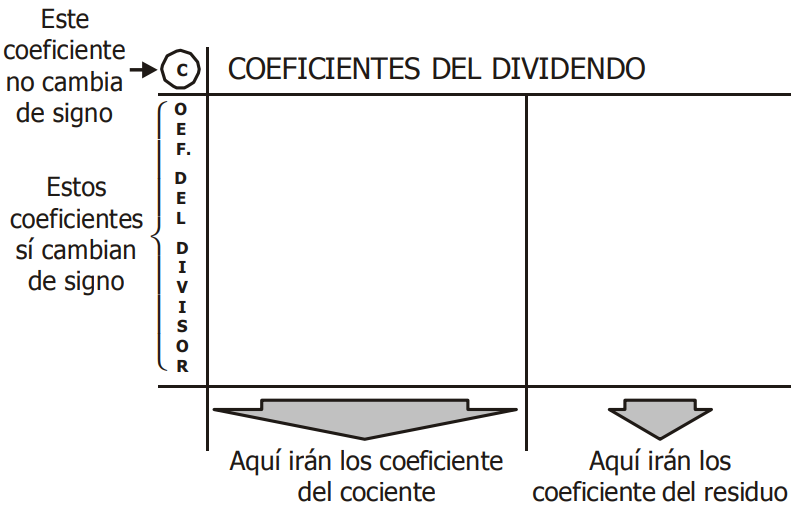
\includegraphics[width=10cm]{images/esquema-grafico-horner}
    \caption{Esquema gráfico del método de Horner.}
    \label{fig:figure}
\end{figure}

Ahora veamos su algoritmo.

\vspace{1cm}\\

\textbf{Algoritmo.}
\begin{enumerate}
    \item Se anotan los coeficientes del dividiendo en la parte superior del cuadro en forma horizontal.
    \item Se anotan los coeficientes del divisor en la parte izquierda del cuadro en forma vertical con los signos cambiados a excepción del primero.
    \item La línea de trazos separa el cociente del resto y para su trazo se considera el grado del divisor.
    En el cociente se cuentan tantos términos como el grado del dividendo menos el grado del divisor más uno.
    \item El primer término del cociente se obtiene dividiendo el primer coeficiente del dividendo entre el primer coeficiente del divisor.
    \item El coeficiente obtenido en el paso anterior se multiplica con los demás coeficientes del divisor con signo opuesto y los resultados se escriben de manera horizontal a partir de la siguiente columna hacía la derecha.
    \item Las cantidades que se encuentran en la segunda columna se suman y el resultado se divide entre el primer coeficiente del divisor, repitiéndose el procedimiento hasta coincidir con la última columna del dividendo.
    \item Para finalizar, se suman directamente las columnas correspondientes al residuo, lo que conformará los coeficientes del polinomio residuo o resto.
\end{enumerate}

\begin{example}
    Dividir $(6x^5 - 20x^4 - 13x^3 + 25x^2 - 12x + 7)$ entre $(3x^2 - x + 1)$
\end{example}
\begin{multicols}{2}
    \begin{solution}
        Acomodamos los polinomios en el gráfico.
        En particular, teniendo cuidado con el divisor.
        La cantidad de columnas para resto esta dada por $(5 - 2) + 1 = 2$.

        Realizamos las operaciones, luego, obtenemos el coeciente $(2x^3 - 6x^2 - 7x + 8)$ y el resto $(3x - 1)$.
        Finalmente, como complemento, podemos expresar el dividendo como
        \[
            (3x^2 - x + 1)(2x^3 - 6x^2 - 7x + 8) + (3x - 1) \qedhere
        \]
    \end{solution}

    \begin{gather*}
        \begin{array}{c|cccc|cc}
             3 & 6 & -20 & -13 & 25 & -12 &  7 \\\hline
            +1 &   &  +2 &  -2 &    &     &    \\
            -1 &   &     &  -6 & +6 &     &    \\
               &   &     &     & -7 &  +7 &    \\
               &   &     &     &    &  +8 & -8 \\\hline
               & 2 &  -6 &  -7 &  8 &  +3 & -1
        \end{array}
    \end{gather*}
\end{multicols}


\subsubsection{Método de Ruffini}

Se recomienda usar el método de Ruffini cuando el divisor tiene la forma $ax \pm b$.
Este método se apoya de un esquema como el siguiente.
\begin{figure}[H]
    \centering
    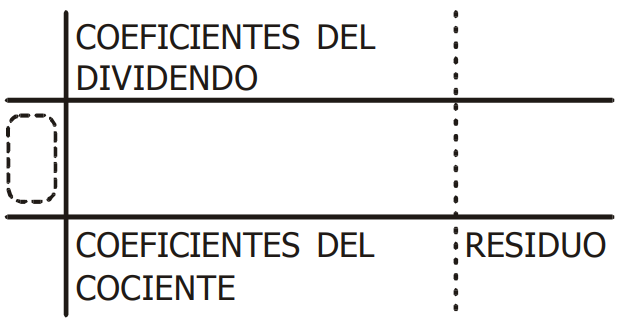
\includegraphics[width=6cm]{images/esquema-grafico-ruffini}
    \caption{Esquema gráfico del método de Ruffini.}
    \label{fig:figure2}
\end{figure}
Donde en el recuadro izquierdo se coloca $\left(-\frac{b}{a}\right)$, es decir, la solución de la ecuación $ax \pm b = 0$.
Cabe mencionar que el método de Ruffini se considera como un caso particular del método de Horner.

\textbf{Algoritmo.}
\begin{enumerate}
    \item Se anotan los coeficientes del dividiendo en forma horizontal y el valor de $\left(-\frac{b}{a}\right)$ en el recuadro izquierdo.
    \item Se baja el primer coeficiente del dividendo y se multiplica por el valor de $\left(-\frac{b}{a}\right)$, el resultado se anota en la siguiente columna, debajo del segundo coeficiente del dividendo.
    \item Se suman las cantidades de la segunda columna y se sigue el mismo procedimiento hasta obtener un término debajo del último coeficiente del dividendo.
    \item El residuo es la suma de cantidades de la última columna.
\end{enumerate}

\begin{example}
    Dividir $(2x^3 + 5x^2 + 10x - 8)$ entre $(x + 3)$.
\end{example}
\begin{multicols}{2}
    \begin{solution}
        Acomodamos los polinomios en el gráfico.
        Realizamos las operaciones, donde obtenemos el cociente $(2x^2 - x + 13)$ y el resto $-47$.
        Finalmente, como complemento, podemos expresar el dividendo como
        \[
            (x + 3)(2x^2 - x + 13) - 47. \qedhere
        \]
    \end{solution}
    \[
        \polyhornerscheme[x=-3]{2x^3 + 5x^2 + 10x - 8}
    \]
\end{multicols}


\subsection{Divisibilidad polinómica}

\begin{theorem.tcb}{Teorema del resto}{}
    Dado un polinomio $P(x)$ con grado $n$ y un número $a \in \R$.
    Si $P(x)$ es dividido por $(x - a)$, entonces el resto de la división es $P(a)$, \ie
    \[
        P(x) = (x - a)Q(x) + r \implies P(a) = r
    \]
    para algún polinomio $Q(x)$.
\end{theorem.tcb}
\begin{proof}
    Por la definición de división podemos escribir $P(x) = (x - a)Q(x) + R(x)$.
    Sabiendo que $\deg R(x) < \deg(x - a) = 1$, necesariamente el resto deber ser un polinomio constante, esto es $R(x) = r$.
    Realizando la evaluación $P(a)$, obtenemos $P(a) = (a - a)Q(a) + R(a) \implies P(a) = R(a)$.
    Como $R(x)$ es constante para toda $x$ tenemos que $P(a) = r$.
\end{proof}

Notemos que el teorema del resto implica al teorema del factor, teorema que ya hemos estudiado.

\begin{theorem.tcb}{Teorema del factor}{}
    Sea $P(x)$ un polinomio y sea $a \in \R$.
    Se cumple que $a$ es raíz de $P(x)$ si y solo si $(x - a)$ es un factor de $P(x)$, \ie
    \[
        P(a) = 0 \iff P(x) = (x - a)Q(x).
    \]
\end{theorem.tcb}
\begin{proof}
    Si tenemos que $P(a) = 0$ y analizamos el residuo en $P(x) = (x - a)Q(x) + R(x)$.
    Por el teorema del resto, sabemos que $P(a) = R(x) = 0$, por tanto $(x - a)$ es un factor de $P(x)$.
    Si tenemos que $P(x) = (x - a)Q(x)$, entonces al evaluar $P(a)$, claramente $P(a) = 0$, por tanto $a$ es una raíz de $P(x)$.
\end{proof}

\begin{theorem.tcb}{Teorema fundamental del Álgebra}{}
    Todo polinomio $P(z) = a_n z^n + a_{n - 1} z^{n - 1} + \cdots + a_1 z + a_0$, donde $n \geq 1$, $a_i \in \C$ y $a_n \neq 0$, tiene al menos una raíz en $\C$.
\end{theorem.tcb}

Desafortunadamente, la demostración del Teorema fundamental del Álgebra es demasiada complicada para nuestro pequeño curso de polinomios.

\begin{theorem.tcb}{}{}
    Todo polinomio de grado $n > 0$ tiene exactamente $n$ raíces, \ie
    \[
        P(x) = a_n x^n + a_{n - 1} x^{n - 1} + \cdots  + a_1 x + a_0 = a_n (x - r_1)(x - r_2) \cdots (x - r_n)
    \]
    donde $r_1, r_2, \cdots, r_n$ son reales o complejos.
\end{theorem.tcb}
\begin{proof}
    Procederemos por \emphtext{inducción matemática} en el grado del polinomio.
    Si el polinomio es de grado 1, el resultado es inmediato.
    Supongamos, entonces, que el resultado es cierto para polinomios con grado $(n - 1)$.

    Consideremos un polinomio $P(x)$ con grado $n$.
    De acuerdo con el Teorema Fundamental del Álgebra, $P(x)$ tiene una raíz $r_1$ y por tanto, por el teorema del factor existe un $Q (x)$ tal que $P(x) = (x - r_1)Q(x)$.
    Como $\deg P(x) = \deg[(x - r_1)Q(x)] \implies n = \deg(x - r_1) + \deg Q(x)$, es decir $\deg Q(x) = (n - 1)$.

    Por la hipótesis de inducción, el polinomio $Q(x)$ tiene exactamente $(n - 1)$ raíces, es decir $Q(x) = C(x - r_2)(x - r_3)\cdots(x - r_n)$.
    Por consiguiente, $P(x) = (x - r_1)Q(x) = C(x - r_1)(x - r_2)\cdots(x - r_n)$ tiene $n$ raíces.
\end{proof}

El resultado que acabamos de demostrar, solo muestra la existencia de las raíces, encontrarlas es otro problema.
Esto lo podemos abordar utilizando las fórmulas de Vieta o la división de polinomios.

\begin{example}
    ¿Es el polinomio $P(x) = x^4 + 2x^3 - 2x^2 + x - 6$ divisible por $(x + 3)$?
\end{example}
\begin{solution}
    Por el teorema del factor, si $(x + 3)$ es factor de $P(x)$, entonces basta probar que $P(-3) = 0$.
    Rápidamente, vemos que $P(-3) = (-3)^4 + 2(-3)^3 - 2(-3)^2 + (-3) - 6 = 0$.
\end{solution}

\begin{example}
    Sea $P(x)$ un polinomio con coeficientes reales.
    Cuando $P(x)$ es dividido por $(x - 1)$, el residuo es 3.
    Cuando $P(x)$ es dividido por $(x - 2)$, el residuo es 5.
    Determinar el residuo cuando $P(x)$ es dividido por el polinomio $(x^2 - 3x + 2)$.
\end{example}
\begin{solution}
    Podemos escribir
    \[
        P(x) = (x^2 - 3x + 2)Q(x) + R(x),
    \]
    donde $R(x)$ es el residuo deseado.
    Ya que $\deg R(x) < \deg(x^2 - 3x + 2) =  2$, existen dos posibles grados para $R(x)$, esto es que sea constante o lineal.
    Para generalizar tomamos el caso lineal, es decir $R(x) = ax + b$ para constantes $a$ y $b$.

    Por otra parte, notamos que los números 1 y 2 son raíces de $(x^2 - 3x + 2)$, en consecuencia tenemos que $P(x) = (x - 2)(x - 1)Q(x) + (ax + b)$.
    Ahora bien, por el teorema del resto, sabemos que $P(1) = 3$ y $P(2) = 5$, esto es
    \begin{align*}
        P(1) &= (1 - 2)(1 - 1)Q(1) + (a + b) = 3\\
        P(2) &= (2 - 2)(2 - 1)Q(2) + (2a + b) = 5
    \end{align*}
    Simplificando, obtenemos el sistema de ecuaciones $a + b = 3\ \land\ 2a + b  = 5$ cuya única solución es $(a, b) = (2, 1)$.
    Finalmente, el residuo deseado es $\boxed{R(x) = 2x + 1}$.
\end{solution}

\begin{example}
    Encontrar el residuo cuando $x^{100} - 4x^{98} + 5x + 6$ es dividido por $x^3 - 2x^2 - x + 2$.
\end{example}
\begin{solution}
    Como el grado del residuo debe ser menor a $\deg{(x^3 - 2x^2 - x + 2)} = 3$, hay tres posibles casos;
    que sea constante, lineal o cuadrático.
    Para tomar en cuenta todos los casos a la vez, diremos que el residuo tiene la forma $R(x) = ax^2 + bx + c$ para constantes $a, b$ y $c$.
    Además, notamos que $x^3 - 2x^2 - x + 2$ puede factorizarse fácilmente como $(x - 2)(x - 1)(x + 1)$.
    Así, podemos escribir la división como
    \[
        x^{100} - 4x^{98} + 5x + 6 = (x - 2)(x - 1)(x + 1)Q(x) + (ax^2 + bx + c),
    \]
    para algún polinomio $Q(x)$ con grado 97.
    Por el teorema del resto, vemos que para $x \in \{-1, 1, 2\}$ se cumple que $\left(x^{100} - 4x^{98} + 5x + 6\right) = R(x)$, \ie
    \begin{align*}
        (-1)^{100} - 4(-1)^{98} + 5(-1) + 6 &= (0)Q(-1) + (a - b + c)\\
        (1)^{100} - 4(1)^{98} + 5(1) + 6 &= (0)Q(1) + (a + b + c)\\
        (2)^{100} - 4(2)^{98} + 5(2) + 6 &= (0)Q(2) + (4a + 2a + c).
    \end{align*}
    Al simplificar, obtenemos el sistema $a - b + c = -2\ \land\ a +  b + c = 8\ \land\ 4a + 2b +  c = 16$.
    Cuya única solución resulta ser $(a, b, c) = (1, 5, 2)$.
    Finalmente, el residuo deseado es $\boxed{R(x) = x^2 + 5x + 2}$.
\end{solution}



\subsection{Ejercicios y problemas}

Ejercicios y problemas para el autoestudio.

\showLine
\begin{multicols}{2}

    \begin{exercise}
        Dado los polinomios $P(x) = 2x^5 + x^4 + ax^2 + bx + c$ y $Q(x) = x^4 - 1$, se sabe que $Q \mid P$.
        Hallar $\dfrac{a + b}{a - b}$.
    \end{exercise}

    \begin{exercise}
        Dado los polinomios $P(x) = 16x^5 + ax^2 + bx + c$ y $Q(x) = 2 x^3 - x^2 + 1$, se sabe que $Q \mid P$.
        Hallar $a + b + c$.
    \end{exercise}

    \begin{exercise}
        Si el polinomio $3x^5 + 6x^3 - 3x$ se le divide entre $x + 1$ se obtiene como resultado un cociente de grado $m$, un término independiente $b$ y un resto $a$.
        Hallar $m + a + b$.
    \end{exercise}

    \begin{exercise}
        Al dividir $x^4 - x^2 - 2x + 1$ entre $x^2 + x + 1$, determine el producto de los términos del cociente.
    \end{exercise}

    \begin{exercise}
        Si $P(x - 2) = x^3 - 10x^2 + 28x - 24$, hallar el resto de dividir $P(x)$ por $x - 3$
    \end{exercise}

    \begin{exercise}
        Si $6x^4 - 11x^2 + ax + b$ dividido entre $3x^2 - 3x - 1$ deja resto $3x + 2$.
        Hallar $a - b$.
    \end{exercise}

    \begin{exercise}
        Si la división de $x^4 + ax^2 + b$ entre $x^2 + x + 1$ es exacta, encuentre los valores de $a$ y $b$ apropiados.
    \end{exercise}

    \begin{exercise}
        Si el polinomio
        \[
            P(x) = ax^4 + bx^3 + cx^2 + 3x + 1
        \]
        se divide por $x^2 - x + 2$ se obtiene un cociente cuya suma de coeficientes es 22 y un resto $R(x) = 10x - 1$, calcular $b + c$.
    \end{exercise}

    \begin{exercise}
        Al dividir el polinomio
        \[
            P(x) = 55x^3 + (166 + b)x - x^2 - 2
        \]
        entre $Q(x) = ax^2 - 39x + 2$, el residuo es de la forma $R(x) = mx$.
        Calcular el valor de $a + b$.
    \end{exercise}

    \begin{exercise}
        Calcular el valor de $a + b$ si $(1 + i)$ es raíz del polinomio $x^5 + ax^3 + b$.
    \end{exercise}

    \begin{exercise}
        ¿Para qué valores de $k$ se cumple que $(x - 2)$ es un factor del polinomio $x^3 + 2kx^2 + k^2 x + k - 3$?
    \end{exercise}

    \begin{exercise}
        Encontrar el resto cuando
        \[
            (x + 3)^5 + (x + 2)^8 + (5x + 9)^{1997}
        \]
        es dividido por $(x + 2)$.
    \end{exercise}

    \begin{exercise}
        Para un polinomio desconocido que deja un resto 2 al dividirlo por $(x - 1)$, y un resto 1 al dividirlo por $(x - 2)$.
        ¿Cuál es el resto que se obtiene si este polinomio es dividido por $(x - 1)(x - 2)$?
    \end{exercise}

    \begin{exercise}
        Encontrar el resto cuando $x^{2006} + x^{2005} + \cdots + x + 1$ es dividido por $(x + 1)$.
    \end{exercise}

    \begin{exercise}
        Sea $F(x) = x^4 + x^3 + x^2 + x + 1$.
        Encontrar el residuo cuando $F(x^5)$ es dividido por $F(x)$.
    \end{exercise}

    \begin{problem}
        Determinar todos los enteros positivos $n$, tales que el polinomio $x^n + x - 1$ sea divisible por el polinomio $x^2 - x + 1$.
    \end{problem}

    \begin{problem}
        ¿Qué valor adquiere $\dfrac{n + 19}{k + 1}$, si la división $\dfrac{x^{19} - nx + k}{x^2 - 2x + 1}$ es exacta?
    \end{problem}
\end{multicols}